\documentclass[conference]{IEEEtran}
\IEEEoverridecommandlockouts
\usepackage{algorithmic}
\usepackage[backend=bibtex,style=ieee,natbib=true]{biblatex}
\usepackage{graphicx}
\usepackage{textcomp}
\usepackage{xcolor}

\addbibresource{main.bib}

\begin{document}

\title{
    COMPSCI 402 --- Artificial Intelligence\\
    Final Report\\
    The Development and Outlook of AI Techniques in The Field of
    Practical Federated Learning on Mobile Devices
}

\author{
    \IEEEauthorblockN{Sichang He}\\
    sichang.he@dukekunshan.edu.cn
}

\maketitle

\begin{abstract}
% TODO: Insert a very brief paragraph to summarize your essay
\end{abstract}

\section{Introduction}

% Briefly introduce your understanding of AI,

The term ``artificial intelligence'' (AI) is used to refer to
artificial machineries that
resembles human intelligence in either the way they function or
the way they behave.
These machineries, or intelligent agents,
are not limited to,
but are often designed and built in the form of computer software programs that
run on general purpose computer hardware.

Machine learning (ML), being a significant topic in AI,
refers to the study of intelligent agents that are able to
adapt to previously unseen situations based on data from the past.
The process where an intelligent agent analyzes data from the past to
prepare its abilities is referred to as ``learning'', or ``training''.
Therefore, the data from the past is referred to as ``training data''.
Once the training is complete,
the agent would be able to make predictions or decisions,
or ``make inferences'',
when facing situations that may potentially not be previously seen.
To achieve ML, the common approach is to build a model,
a program that implements some mathematical function,
and train this model by altering the parameters in the function.

% provide an overview of the application of the AI in your research area.
% For example, you can discuss the current development trend and
% provide a roadmap of the development of AI techniques in your research area.

Federated learning (FL), first proposed in 2016, is an ML technique that
allows distributed intelligent agents to collaborately train a model using
their local data~\cite{mcmahan2017communication}.
These private data are kept local,
therefore FL is suitable for scenarios where
the training data cannot be shared to a central intelligent agent due to
privacy restrictions.

The increasing need to train ML models for business,
the rising awareness of data privacy among individuals,
and the improving laws of governments contribute to
the growing applications of FL.
FL is a compelling option for companies to train ML models using users' data
without breaking some of the privacy laws.

The applications of FL broadly concerns with situations where
the private data that individual intelligent agent possesses are in
the center of the problem.
Some of the earliest practical applications of FL are proposed
in~\cite{bonawitz2019towards},
including selecting and ranking items, suggesting relevant content,
and next-word prediction for smart keyboard on mobile devices.
In all these applications,
the private data from the users' interactions with
the keyboard are in the center of the problems.
Since then, a large portion of practical applications of FL have been
focusing on applications on mobile devices.
For example, vision-based product quality inspection~\cite{bharti2022edge} using
an iOS application and
SMS spam classification on Android devices~\cite{sriraman2022device}.

Despite the advantages of mobile FL on paper,
the practical applications of FL on mobile devices are still limited.
FL is proposed in as early as 2016~\cite{mcmahan2017communication},
and the first effective and well-known application of FL
was announced in 2019~\cite{bonawitz2019towards},
yet, in 2023, FL applications are still rare to see.
The reason is that practical FL faces many challenges such as
privacy security, training efficiency and performance issues,
and heterogeneity problems~\cite{wen2023survey}.

\section{The General Procedure of Federated Learning}

Generally, FL involves a distributed system that
consists of two parties of intelligent agents and
four phases per training iteration,
as illustrated in Fig.~\ref{fig:general-fl}.
The two parties are the central server and the clients.
From the perspective of the ML models being trained,
for each iteration,
the global model is distributed to the clients from the central server;
then, the clients train it locally using local training data;
after local training,
the clients send the trained local models back to the central server;
finally, these local models are aggregated into a new global model,
and the process is potentially repeated for the next new iteration.

The most typical FL algorithm, \verb|FedAvg|,
is proposed in~\cite{mcmahan2017communication}.
We assume $K$ clients, where each client $k$ has a partition $P_k$ of
the total training data ($k \in \{1, 2, \dots, K\}$) as their local data.
For efficiency,
in each iteration $t$ of the training process,
the central server randomly samples $C$ clients for local training.
Each selected client $k$ obtains the parameters $w^{(t)}$ of
the latest global model from the server,
and then train the model locally using their local data $P_k$ to
produce a new local model with parameters $w_k^{(t+1)}$.
The objective of this local training process is to minimize the loss $L$ of
the model with parameters $w_k$ for partition $P_k$:
\begin{equation}
    \min_{w_k} L(P_k;w_k).
\end{equation}
And, the objective to optimize the global model is
\begin{equation}
    \min_{w} \frac{\sum_k |P_k|L(P_k;w)}{\sum_k |P_k|}
\end{equation}
where $|P_k|$ is the size of partition $P_k$.
To approach this objective,
\verb|FedAvg| aggregates the parameters of local models by
taking the weighted average:
\begin{equation}
    w^{(t+1)}=\sum_k \frac{|P_k|}{\sum_k |P_k|}w_k^{(t+1)}.
\end{equation}
This algorithm has been shown to be effective and practical in experiments.

The typical settings for the original \verb|FedAvg| can be changed in
various ways for different FL needs.
For example,
the sampling of clients can be changed to a function based on
each client's properties instead of being random,
and the number of clients sampled each iteration could vary.
The local training could be customized just like any regular ML training.
And, the aggregation of the local parameters could use another function.
Scheduling techniques are developed to overcome the problem where
a small number of clients lag behind all other clients,
known as
``the straggler issue''~\cite{chen2020asynchronous,zheng2017asynchronous}.
For example, instead of using strict iterations,
the training process could be asynchronous~\cite{zhu2022online}.
All these techniques are developed to improve the performance of FL
so it can be practical.

Model personalization is another popular variant of FL.
While FL generally aims to train a global model,
in model personalization,
local models are adjusted using each user's data to
adapt to the each specific user.
Therefore, model personalization excels general FL when
facing high statistical heterogeneity among the users~\cite{kulkarni2020survey}.
Model personalization also reduces some restrictions and difficulties that
general FL faces.
For example,
we usually aim to update most or all layers in general FL,
but it is common to only update the last layer of neural networks in
transfer learning,
a type of model personalization.
By only updating the last layer,
model personalization can remain efficient even when
the neural network used is deep;
in contrast, the computational complexity in back propagation for
deep neural networks makes it unsuitable for general FL on mobile devices.
Therefore, general FL either requires smaller models to be used,
or partial updates,
or other techniques to be applied so it does not train the whole model.

\begin{figure}
\centerline{
    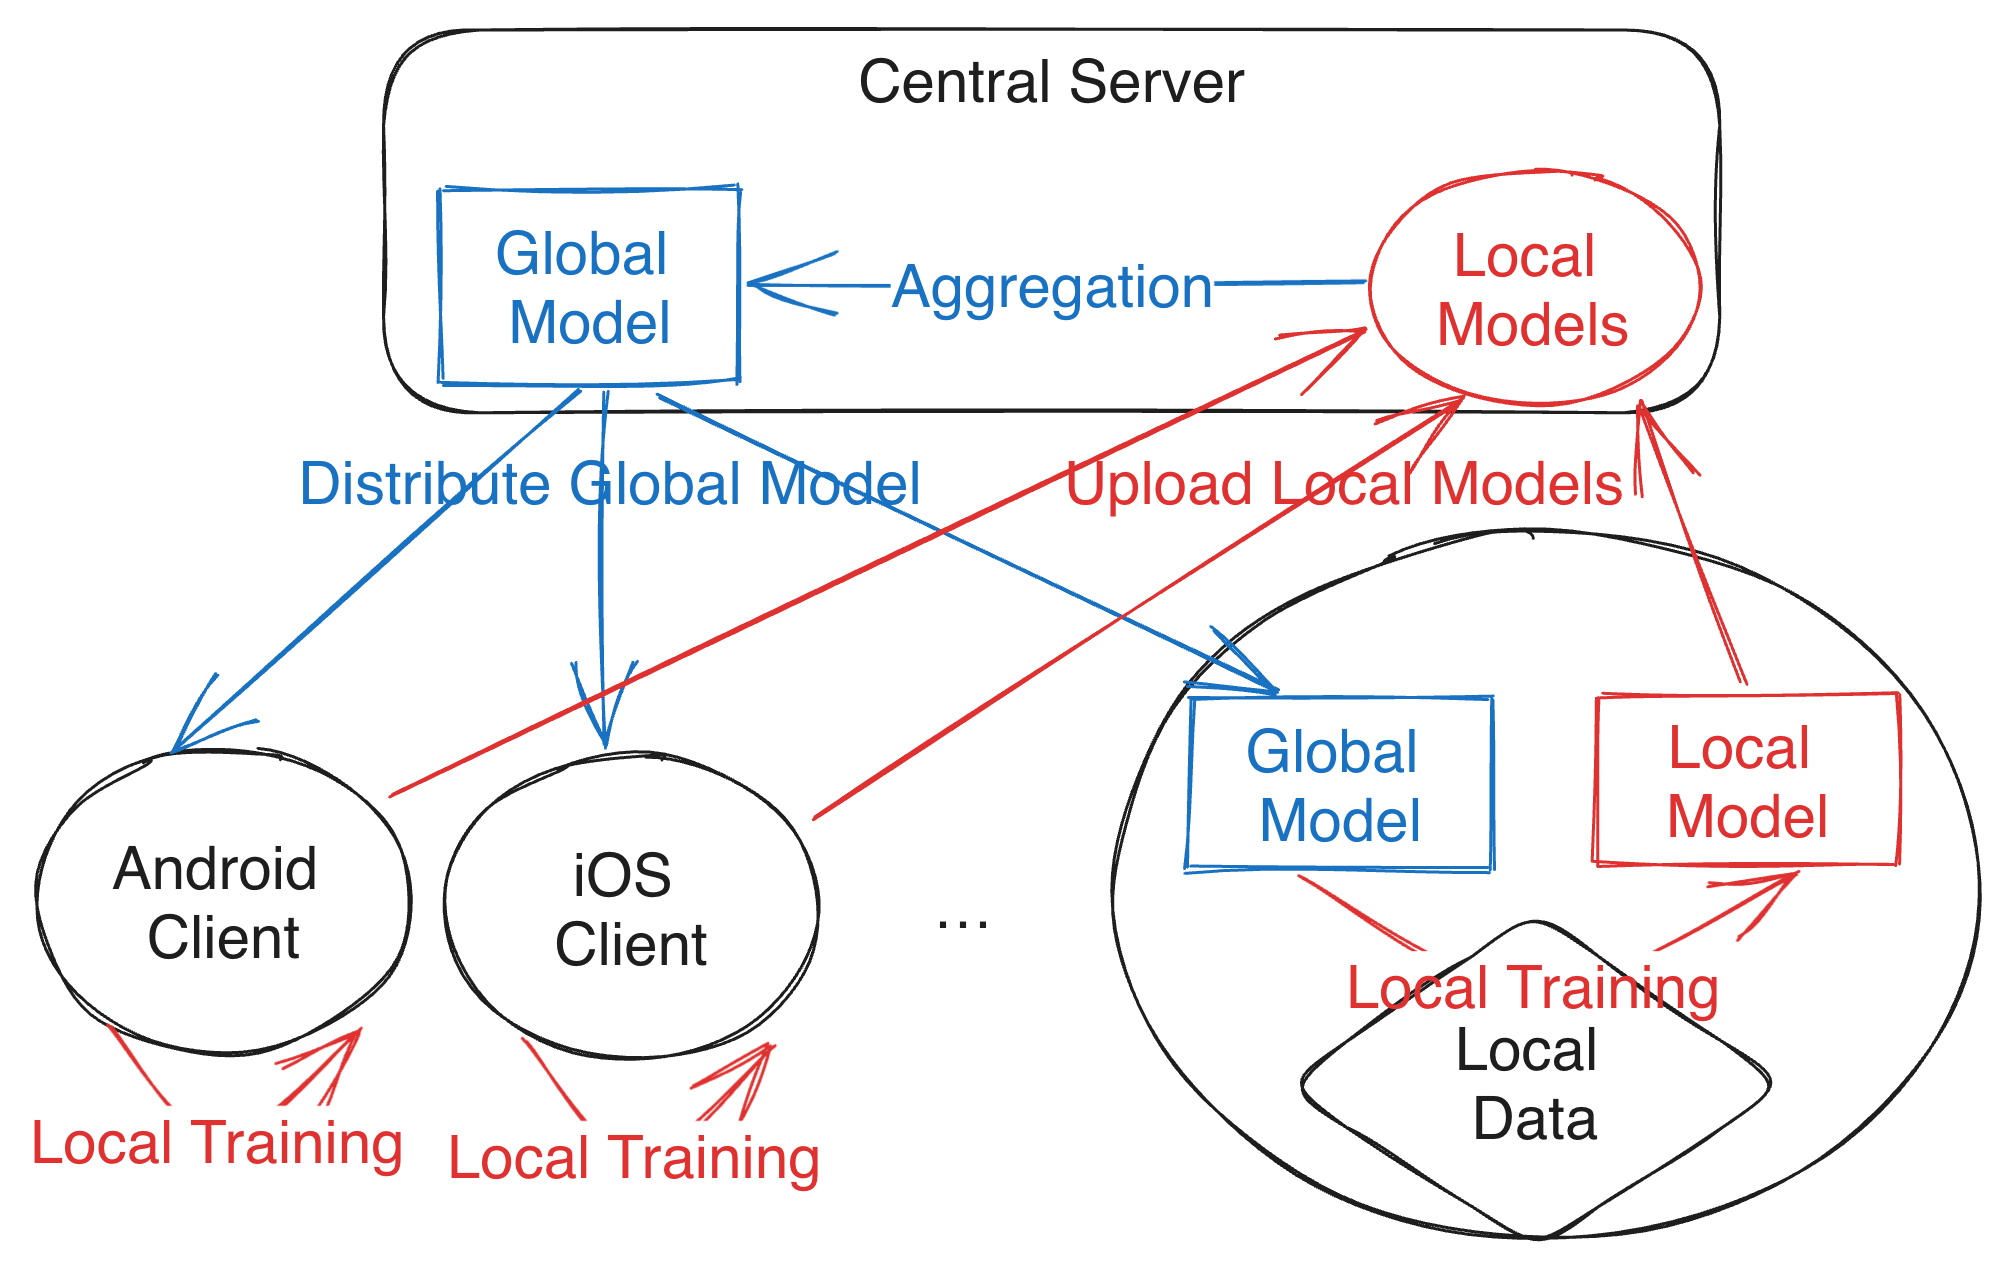
\includegraphics[width=0.5\textwidth]{general-fl.png}
}
\caption{General Procedure of FL for Mobile Devices.}
\label{fig:general-fl}
\end{figure}

\section{Scheduling}

\section{Communication}

\section{On-Device Training}

Most FL systems utilize existing mobile ML frameworks to
support on-device training.
Google's TensorFlow Lite~\cite{tensorflow2015-whitepaper} for Android is
a popular choice due to its flexibility and
its maturity for on-device training.
For example, TensorFlow Lite is used by FL frameworks such as~\cite{
    beutel2020flower,mathur2021ondevice,kourtellis2020flaas,katevas2022flaas}
for their Android support.
In contrast, Apples's Core ML~\cite{coreml} is less popular because
it is much less user-friendly.
Core ML is only used by a few FL frameworks such as
Flower~\cite{beutel2020flower} for iOS support,
and is more commonly used for specific applications
such as this vision-based quality inspector application~\cite{bharti2022edge}.
Third-party solutions for these mobile operating systems are less commonly used.
For example, FedML~\cite{he2020fedml} uses
the MNN ML framework~\cite{jiang2020mnn} for its on-device training on Android.

Some systems choose to adopt solutions that are not specifically designed for
mobile ML,
including web-based and UNIX-environment-based solutions.
For example,
TensorFlow.js is capable of running inside a browser on mobile devices or
a webview inside mobile applications~\cite{smilkov2019tensorflow}.
The usage of TensorFlow.js by~\cite{sriraman2022device} resulted in
difficulties in testing,
but~\cite{palanisamy2021spliteasy} shows the advantages of TensorFlow.js on iOS
by integrating it into a React Native application for split learning.
Another example is FedScale~\cite{lai2022fedscale},
which uses Termux, a UNIX console on Android,
to run TensorFlow directly.
FedScale's solution is only suitable for its benchmarking purposes because
it requires the Termux application to run and
cannot be embedded.

\section{TODO: Main Body}

TensorFlow Federated~\cite{tensorflow2015-whitepaper} is oriented to
provide infrastructure for production-level FL on smartphones.
It is widely used for simulation for its rich feature including
decentralized simulation using gRPC,
but it does not have on-device training support~\cite{kholod2020open}.

FedML~\cite{he2020fedml} is a FL as a Service (FLaaS).
It uses MNN for its training on Android,
and it has not provided an iOS SDK.

Flower~\cite{beutel2020flower,mathur2021ondevice}
only provides a communication layer and
leaves the training implementation to the users.
For the training implementation,
its Android example depends on TensorFlow Lite and
its iOS example depends on Core ML.

Syft~\cite{ryffel2018generic,Ziller2021,hall2021syft}
proposes a custom training process and
offers implementations for both Android and iOS,
but it is low-performance and only uses CPU.

PaddlePaddle~\cite{ma2019paddlepaddle} by Baidu is
also mainly for simulations oriented to production.
It supports inference on Android.

FATE~\cite{liu2021fate} is mainly for production-level simulations.
TODO: read again.

OpenFL~\cite{patrick2022openfl} is also mainly for simulations.
TODO: read again.

FedScale~\cite{lai2022fedscale} leans towards benchmarking.
It supports Android via a UNIX environment.

Project Florida~\cite{madrigal2023project}
is a production-ready FLaaS by Microsoft.
Its Android training is marketed as accelerated,
and its iOS training is not mentioned.

% (You can use table to summarize the features of existing methods;
% or you can conduct the comparative study by
% testing some state-of-the-art methods on your selected dataset.)

\begin{table}[htbp]
\caption{Table Type Styles}
\begin{center}
\begin{tabular}{|c|c|c|c|}
\hline
\textbf{Table}&\multicolumn{3}{|c|}{\textbf{Table Column Head}} \\
\cline{2-4} 
\textbf{Head} & \textbf{\textit{Table column subhead}}& \textbf{\textit{Subhead}}& \textbf{\textit{Subhead}} \\
\hline
copy& More table copy$^{\mathrm{a}}$& &  \\
\hline
\multicolumn{4}{l}{$^{\mathrm{a}}$Sample of a Table footnote.}
\end{tabular}
\label{tab1}
\end{center}
\end{table}

\section{Discussion}

% TODO: Provide an outlook on the development of AI technology in
% your research area based on your knowledge of your research area and
% your understanding of AI.
% You can discuss some open challenges and try to
% provide the corresponding potential solutions or
% discuss the potential research directions.

Security remains a critical concern in FL.
Attacks to FL systems to reverse engineer the training data have been
demonstrated to be practical~\cite{sun2019really}.
Mechanism that increase anonymity and
reduce the risk of successful attacks have been proposed and implemented.
For example, multi-party computing,
differential privacy~\cite{dwork2006differential} and
secure aggregation are
adopted by many production-level FL frameworks and
their effectiveness has been demonstrated.

However, the real-world application on mobile devices still faces a fundamental
issue of trust.
After the mobile applications obtain the training data,
there is no obvious way to verify whether the data are used for FL,
or are in fact sent to a central server.
Companies may well use FL to cover their direct data collection under the hood.

\printbibliography

% TODO: at least 10 references,
% 50\% references should be published within 5 years,
% blogs/website/news reports should be less than 10\%.

\end{document}
